% pfgmanual -> 22.5 Plotting a Function
% https://tex.stackexchange.com/questions/193259/what-is-the-easiest-way-to-accomplish-textual-tick-labels-in-tikz

\begin{tikzpicture}[circuit ee IEC, thick]
    \draw [o-] (0, 0) node[above] {$A$} to (1, 0) ;
    \draw (1, 0) to (1, 1) to[resistor={info=$R_1$}] (3, 1)
      (1, 0) to (1, -1) to[resistor={info=$R_2$}] (3, -1) to (3, 1);
    \draw (3, 0) to[resistor={info=$R_3$}] (4.5, 0);
    \draw (4.5, 0) to[resistor={info=$R_4$}] (6, 0);
    \draw [-o] (6, 0) to ++(0.5, 0) node[above] {$B$};
\end{tikzpicture}


\begin{tikzpicture}[circuit ee IEC, thick]
    \draw [o-] (0, 0) node[above] {$A$} to (1, 0) ;
    \draw (1, 0) to (1, 1) to[resistor={info=$R_1$}] (2.5, 1) to[resistor={info=$R_2$}] (4,1)
          (1, 0) to (1, -1) to[resistor={info=$R_3$}] (4, -1) to (4, 1);
    \draw (4, 0) to[resistor={info=$R_4$}] (5.5, 0);
    \draw [-o] (5.5, 0) to ++(0.5, 0) node[above] {$B$};
\end{tikzpicture}




\begin{tikzpicture}[domain=0:24, xscale=0.2, yscale=0.3]
\draw[thin,color=gray,densely dashed,xstep=5,ystep=2] (0.0,0.0) grid (23,11.5);
\draw[-{Latex},semithick] (0,0) -- (24,0) node[below] {$t, \text{c}$};
\draw[-{Latex},semithick] (0,0) -- (0,12) node[left] {$v, \text{м/с}$};
\draw[very thick] (0,2) -- (22,10.8);
% \draw[very thick] plot (\x,{2 + 0.4 * \x});

\foreach \x in {5,10,15,20} \draw (\x,0) node[below] {$\x$};
\foreach \y in {0,2,4,6,8,10} \draw (0,\y) node[left] {$\y$};
\end{tikzpicture}


\begin{tikzpicture}[domain=0:24, xscale=0.2, yscale=0.15]
\draw[thin,color=gray,densely dashed,xstep=5,ystep=5] (0.0,0.0) grid (23,27);
\draw[-{Latex},semithick] (0,0) -- (24,0) node[below] {$t, \text{c}$};
\draw[-{Latex},semithick] (0,0) -- (0,28) node[left] {$v, \text{м/с}$};
\draw[very thick] (0,5) -- (22,27);
% \draw[very thick] plot (\x,{2 + 0.4 * \x});

\foreach \x in {5,10,15,20} \draw (\x,0) node[below] {$\x$};
\foreach \y in {0,5,10,15,20,25} \draw (0,\y) node[left] {$\y$};
\end{tikzpicture}


\begin{tikzpicture}[domain=0:20, xscale=0.2, yscale=0.01]
\draw[-{Latex[scale=1.3]},semithick] (0,0) -- (25,0) node[below] {$\uptau, \text{мин}$};
\draw[-{Latex[scale=1.3]},semithick] (0,0) -- (0,450) node[left] {$t, \celsius$};
\draw[very thick] (0,27) -- (15,327) -- (22,327);
% \draw[very thick] plot (\x,{2 + 0.4 * \x});

\foreach \x in {5,10,15} \draw (\x,0) -- +(0, 10) -- +(0, -10) -- +(0, 0) node[below] {$\x$};
\foreach \y in {27,127,227,327} \draw (0,\y) -- +(0.5, 0) -- +(-0.5, 0) -- +(0, 0) node[left] {$\y$};
\draw[thin,densely dashed]
    (5,0) -- (5,127) -- (0,127)
    (10,0) -- (10,227) -- (0,227)
    (15,0) -- (15,327) -- (0,327)
;
\draw (0,0) node[below left] {$0$};
\end{tikzpicture}


\begin{tikzpicture}[domain=0:2]
    \draw[-{Latex},semithick] (0,0) -- (2,0) node[below] {$t, \text{c}$};
    \draw[-{Latex},semithick] (0,0) -- (0,2) node[left] {
    \fbox{?}};
    \draw[very thick] (0,1.3) -- (1.5,1.3);
    \draw (0,0) node[left] {$0$};
\end{tikzpicture}

\begin{tikzpicture}[domain=0:2]
    \draw[-{Latex},semithick] (0,0) -- (2,0) node[below] {$t, \text{c}$};
    \draw[-{Latex},semithick] (0,0) -- (0,2) node[left] {
    \fbox{?}};
    \draw[very thick] (0,0.5) -- (1.5,1.7);
    \draw (0,0) node[left] {$0$};
\end{tikzpicture}


\begin{tikzpicture}[domain=0:6.5, xscale=0.5, yscale=0.5]
\draw[-{Latex},thick] (-0.5,0) -- (7,0) node[below] {$t$};
\draw[-{Latex},thick] (0,-0.5) -- (0,8) node[left] {$x$};
% \draw[very thick] (0,2) -- (22,10.8);
\draw[very thick] plot (\x,{(\x-1.5) * (\x - 4) / 2});

\draw[thin,densely dashed]
    (1.5,0) -- +(0, 0.2) -- +(0, -0.2) -- +(0, 0) node[below] {$t_1$}
    (2.75,-0.78125) -- (2.75,0) node[above] {$t_2$}
    (4,0) -- +(0, 0.2) -- +(0, -0.2) -- +(0, 0) node[below] {$t_3$}
    (0,3) -- +(0.2, 0) -- +(-0.2, 0) -- +(0, 0) node[left] {$x_1$}
;
\draw (0,0)  node[below left] {$0$};
\end{tikzpicture}


\begin{tikzpicture}[domain=0:7, xscale=0.5, yscale=0.5]
\draw[-{Latex},thick] (-0.5,0) -- (7,0) node[below] {$t$};
\draw[-{Latex},thick] (0,-5) -- (0,3) node[left] {$x$};
\draw[very thick] plot (\x,{- (\x-1.5) * (\x - 5) / 2});

\draw[thin,densely dashed]
    (1.5,0) -- +(0, 0.2) -- +(0, -0.2) -- +(0, 0) node[above] {$t_1$}
    (3.25,1.53125) -- (3.25,0) node[below] {$t_2$}
    (5,0) -- +(0, 0.2) -- +(0, -0.2) -- +(0, 0) node[above] {$t_3$}
    (0,-3.75) -- +(0.2, 0) -- +(-0.2, 0) -- +(0, 0) node[left] {$x_1$}
;
\draw (0,0)  node[below left] {$0$};
\end{tikzpicture}

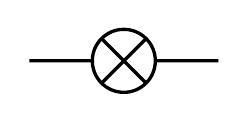
\begin{tikzpicture}[scale=2]
\draw[very thick] (0,0) circle [radius=0.2]
    (-0.141,-0.141) -- (0.141,0.141)
    (-0.141,0.141) -- (0.141,-0.141)
    (-0.6,0) -- (-0.2,0)
    (0.6,0) -- (0.2,0)    
;
\end{tikzpicture}

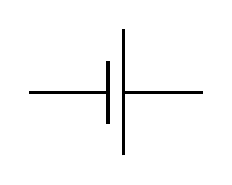
\begin{tikzpicture}[scale=2]
\draw[ultra thick] (0,-0.2) -- (0,+0.2);
\draw[very thick] (-0.5,0) -- (0,0)
    (0.1,-0.4) -- (0.1,0.4)
    (0.1,0) -- (0.6,0)
;
\end{tikzpicture}

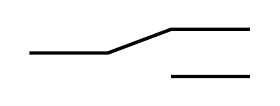
\begin{tikzpicture}[scale=2]
\draw[very thick] (0,0) -- (0.5,0) -- (0.9,0.15) -- (1.4,0.15) (0.9,-0.15) -- (1.4, -0.15)
;
\end{tikzpicture}
